\subsubsection{Overview of the Report}
This report aims to analyze the relationship between urban design features of the city and crime analysis in Berlin. Through data-driven methodologies and spatial analysis, we seek to identify correlations, pinpoint hotspots, and provide actionable insights to inform policy-making and urban planning efforts.



\subsubsection{Population Overview}
As of December 31, 2022, Berlin's population stood at 3,755,251 residents, with 2,920,902 being German nationals and 834,349 foreigners, accounting for 22.2\% of the total population.

\begin{figure}[h]
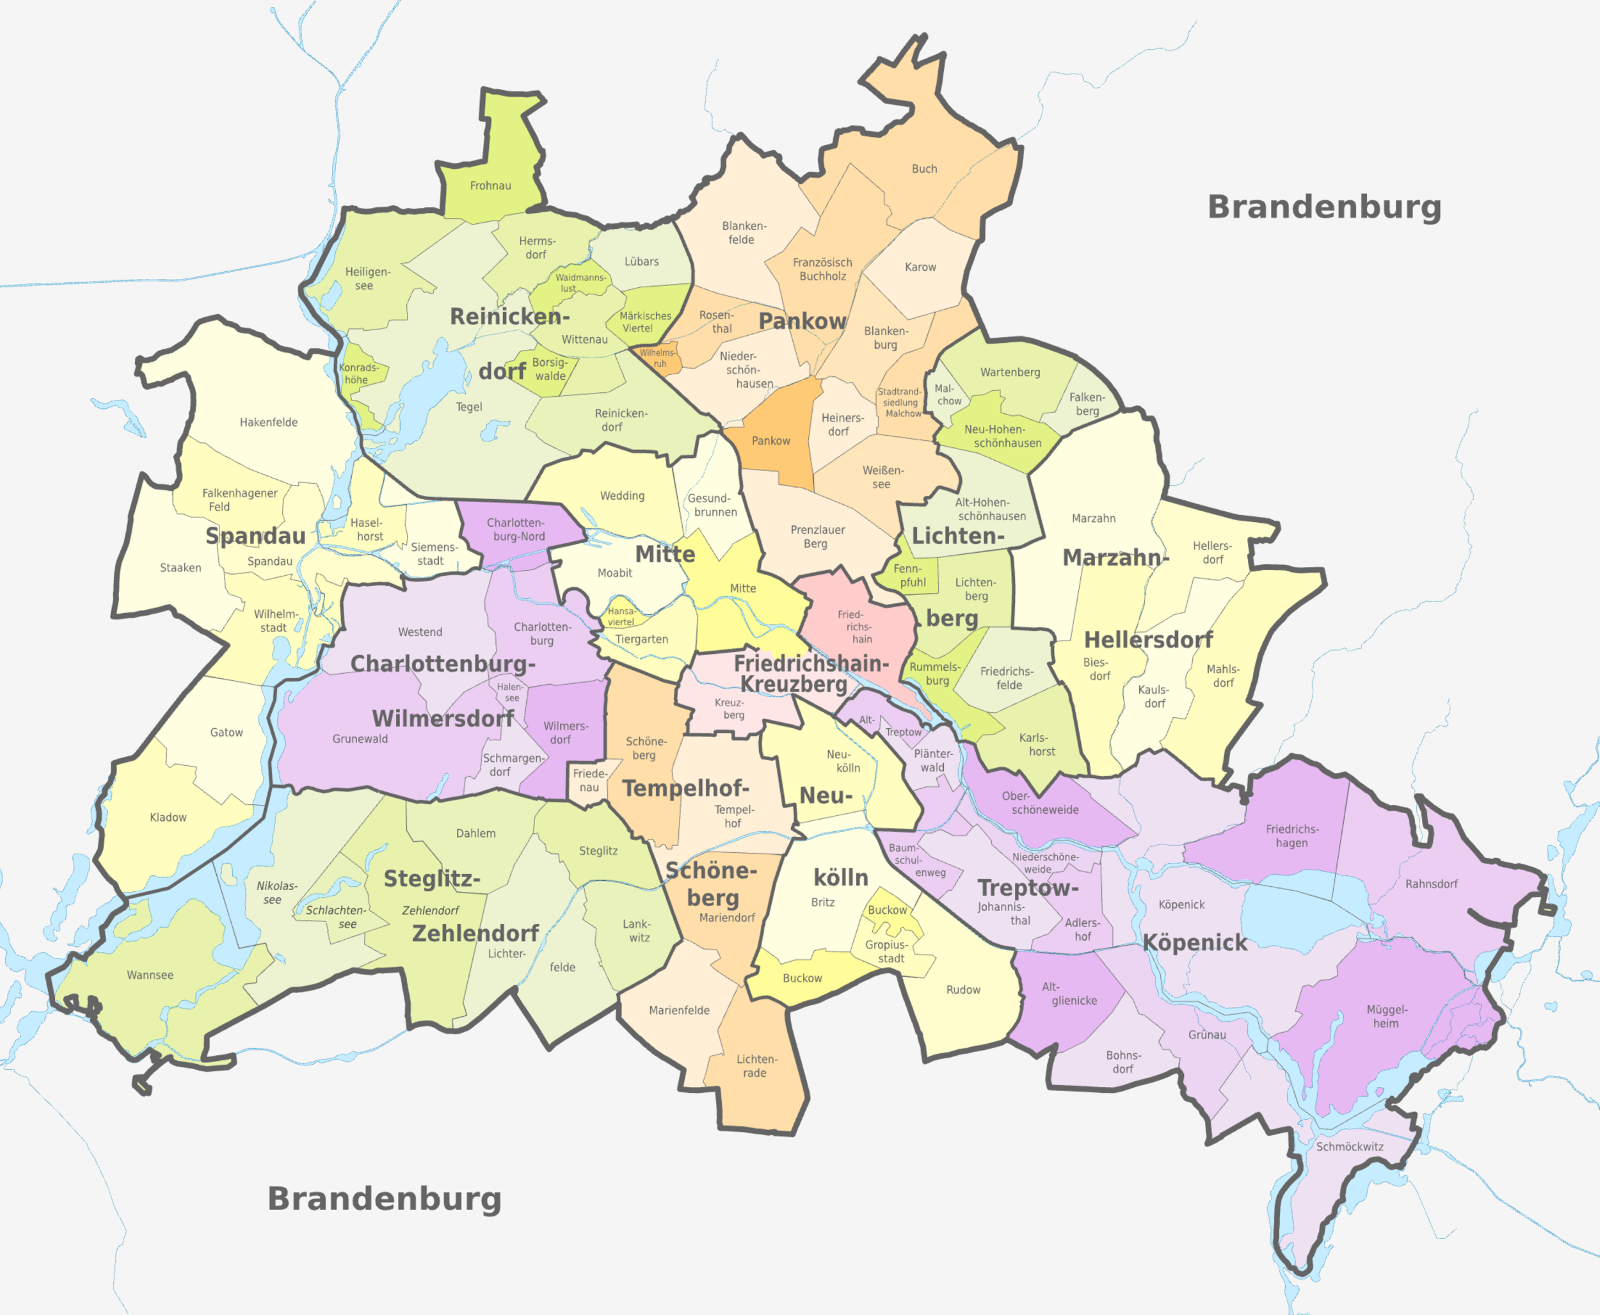
\includegraphics[width=0.7\textwidth]{./figures/intro_rishabh/1_0.png}
    \caption{The image represents Berlin and its 12 boroughs which makes up of 97 localities.}
    \label{fig:districts}
\end{figure}



\subsubsection{Berlin District Map}
As of 2012, the twelve boroughs are made up of a total of 97 officially recognized localities (Ortsteile).

\subsection{Data Collection}
Urban crime data is systematically gathered from police websites, press portals, and news outlets like MoPo using a Python-based web crawler. This includes capturing crucial details such as incident dates, times, locations, and crime types.

The collected data is structured and stored in Neo4j, a robust graph database renowned for managing interconnected data effectively (Figure \ref{fig
}). In Neo4j, nodes represent various entities such as crime incidents, individuals involved (e.g., perpetrators, victims), and specific geographical locations. Relationships between these entities are modeled as edges in the graph, illustrating connections such as repeated criminal activities or spatial associations.

\begin{figure}[h]
	\centering
	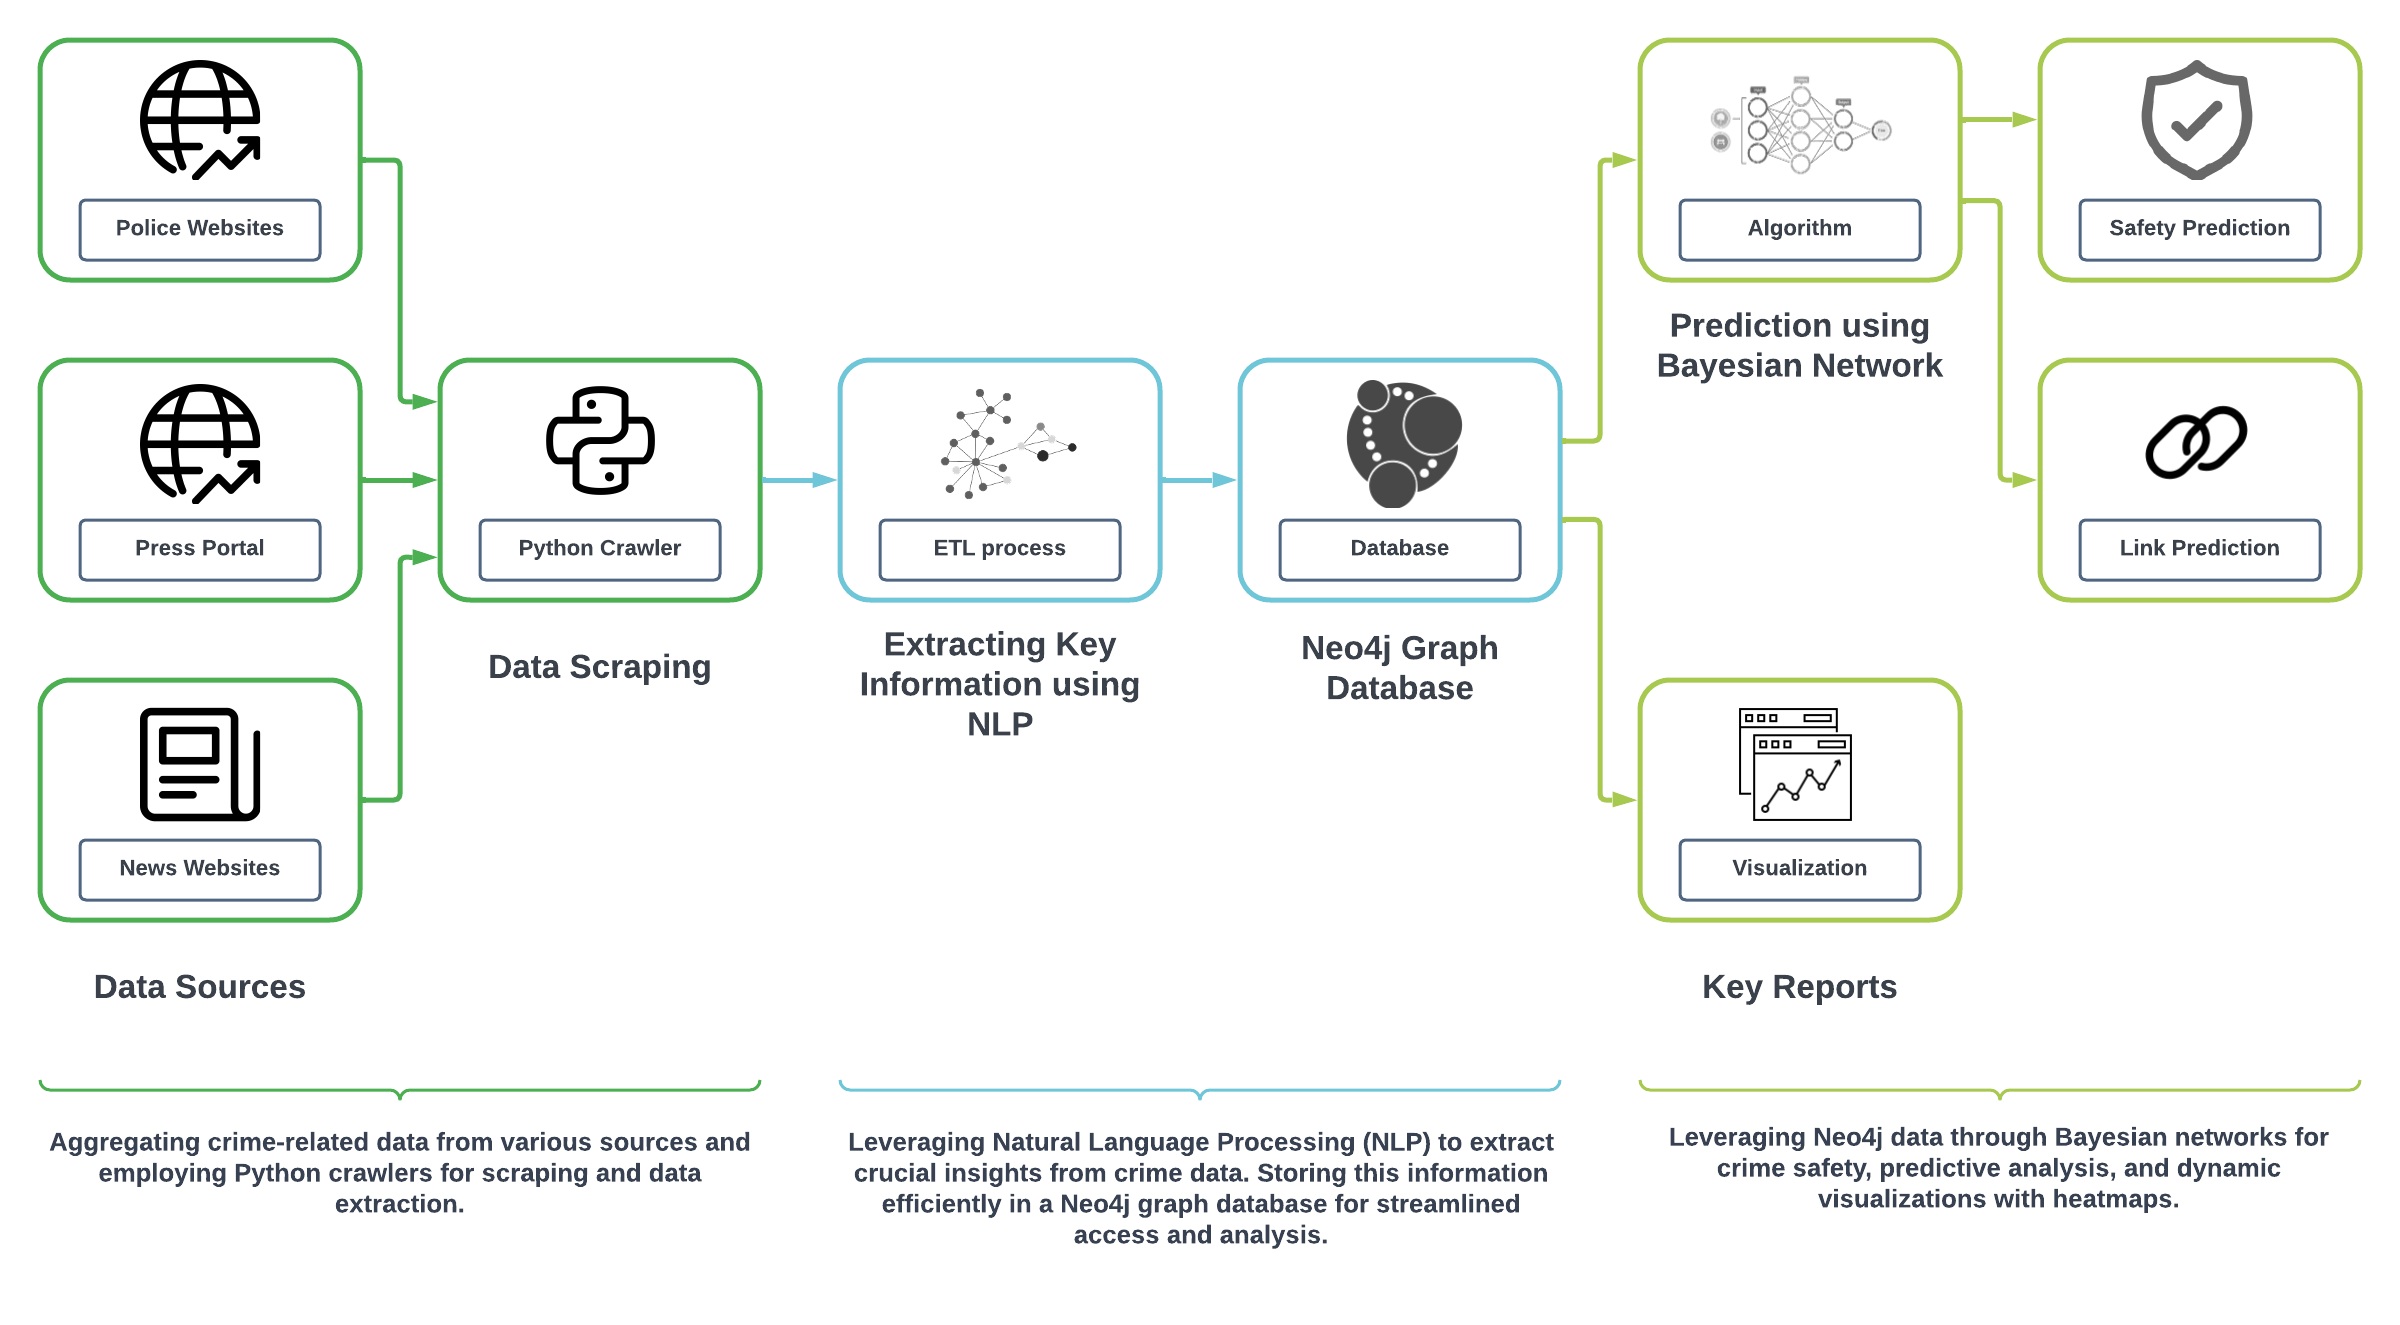
\includegraphics[width=\textwidth]{./figures/intro_rishabh/Data_urbview.png}
	\caption{Database Overview}
	\label{fig}
\end{figure}

Utilizing Neo4j's advanced querying capabilities, we conduct comprehensive analyses to identify hidden patterns and correlations within the urban crime dataset. This analytical approach enables the creation of detailed crime heat maps and the development of predictive models. These visualizations, implemented using tools like Power BI and Python, provide actionable insights for urban planners and law enforcement agencies. They facilitate targeted interventions and enhance strategies for crime prevention, contributing to safer urban environments.
\subsection{Crime Analysis}

\subsubsection{Analysis by Type of Crime}
An analysis of crime categories in Neukölln reveals the following distribution: theft leads with 398 incidents (30.59\%), followed by damage to property at 246 incidents (18.91\%), sexual abuse at 193 incidents (14.83\%), injury at 184 incidents (14.14\%), robbery at 144 incidents (11.07\%), harassment at 116 incidents (8.92\%), and murder at 20 incidents (1.54\%).

\begin{figure}[h]
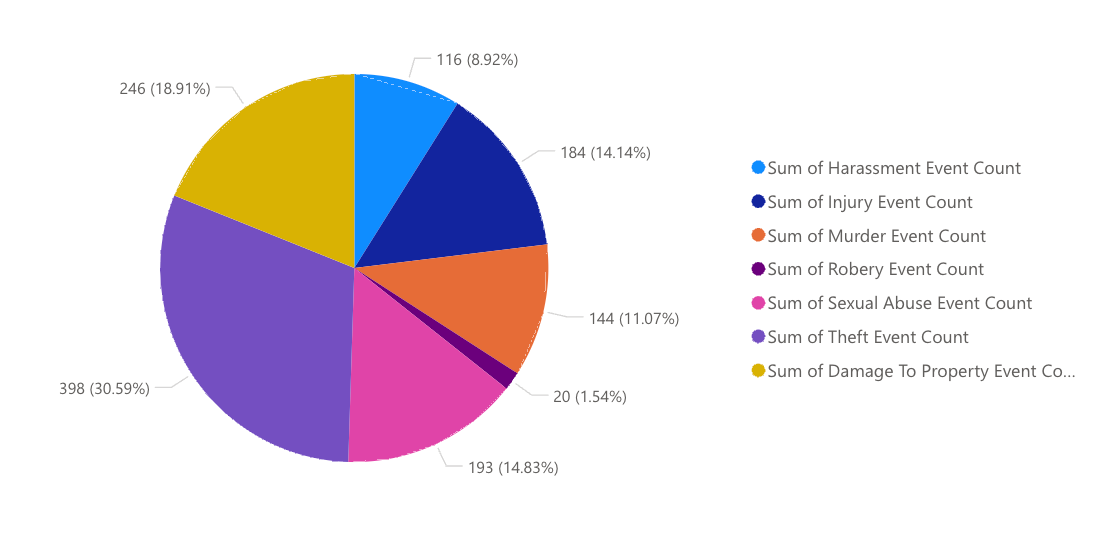
\includegraphics[width=\textwidth]{./figures/intro_rishabh/1_1.png}
    \caption{The above pie chart represents the crime by percentage share based on their type}
    \label{fig:districts}
\end{figure}

\subsubsection{Crime Ranking and Distribution Year on Year}
Neukölln ranks third in crime incidence among Berlin districts, with a total of 678 recorded incidents from 2010 to 2024, accounting for approximately 6.59\% of all crime in Berlin. This significant share highlights Neukölln as a hotspot for criminal activity within the city. The data indicates a consistent pattern of crime, necessitating focused law enforcement efforts.

\begin{figure}[h]
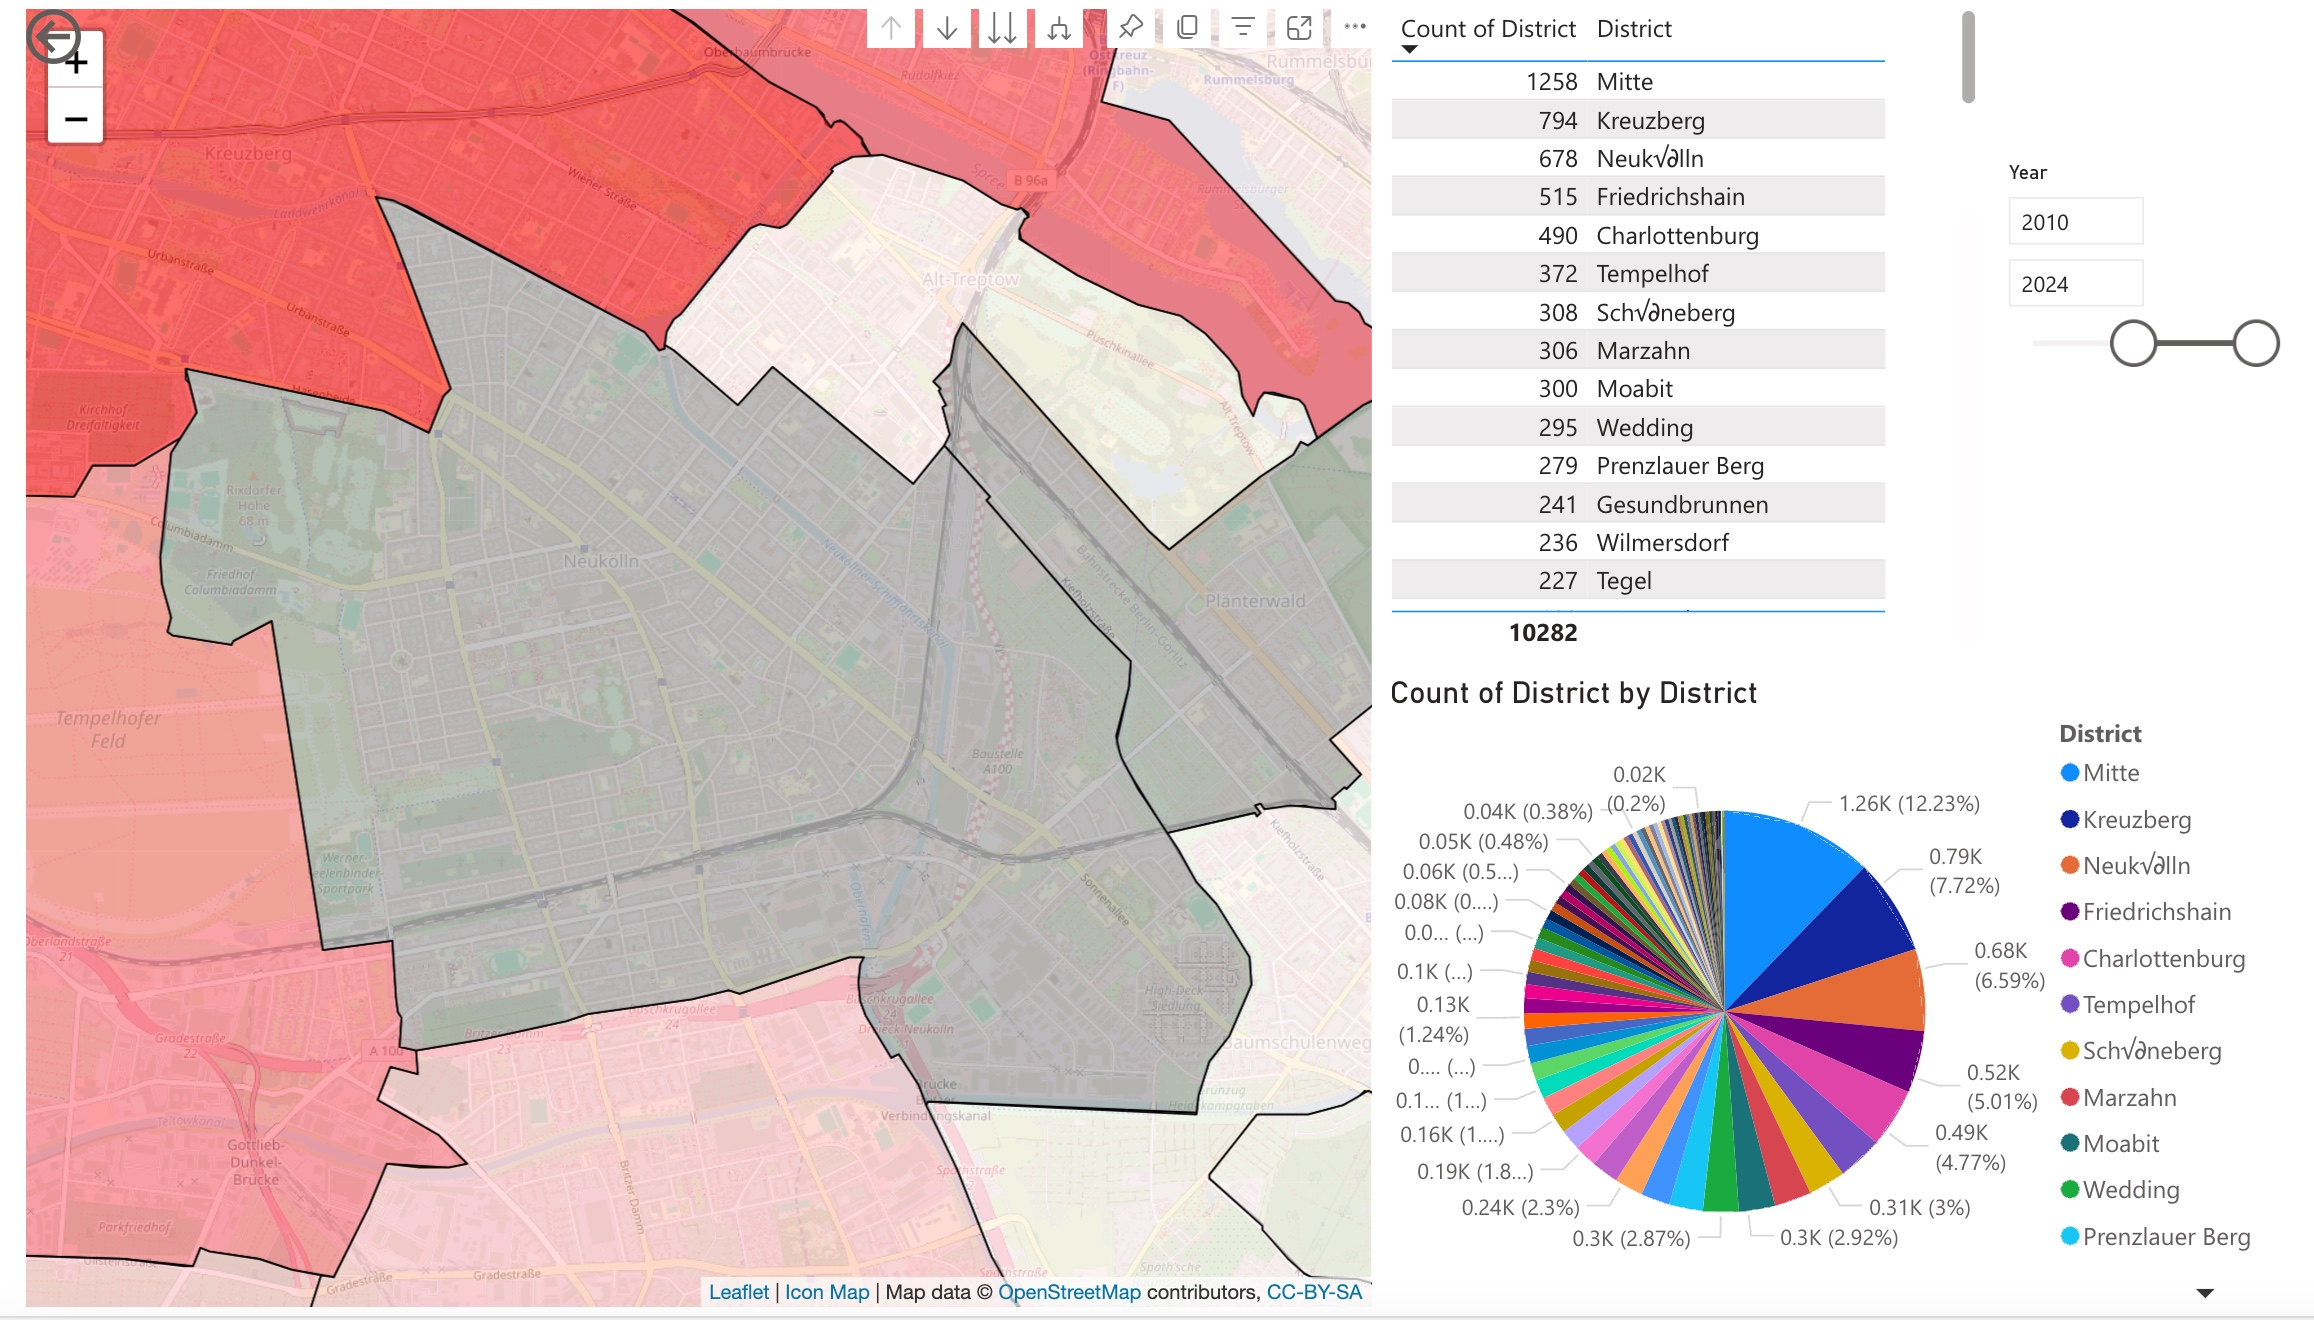
\includegraphics[width=\textwidth]{./figures/intro_rishabh/1_2.jpg}
    \caption{The image shows crime year on year in the city neighbourhoods and their crime share compared to other neighbourhoods in the city.}
    \label{fig:districts}
\end{figure}

\paragraph{The high crime rate in Neukölln can be attributed to its dense population, diverse demographic profile, and the presence of numerous commercial areas. Social and economic disparities also play a role. Effective strategies, including increased police patrols and community engagement programs, are essential to address and reduce crime in this district.}

\subsubsection{Crime Distribution by Time of Day}
An analysis of 361 recorded incidents in Neukölln shows a significant concentration of crimes during noon (179 incidents) and evening (165 incidents), with fewer crimes in the morning (11 incidents) and night (6 incidents).

\begin{figure}[h]
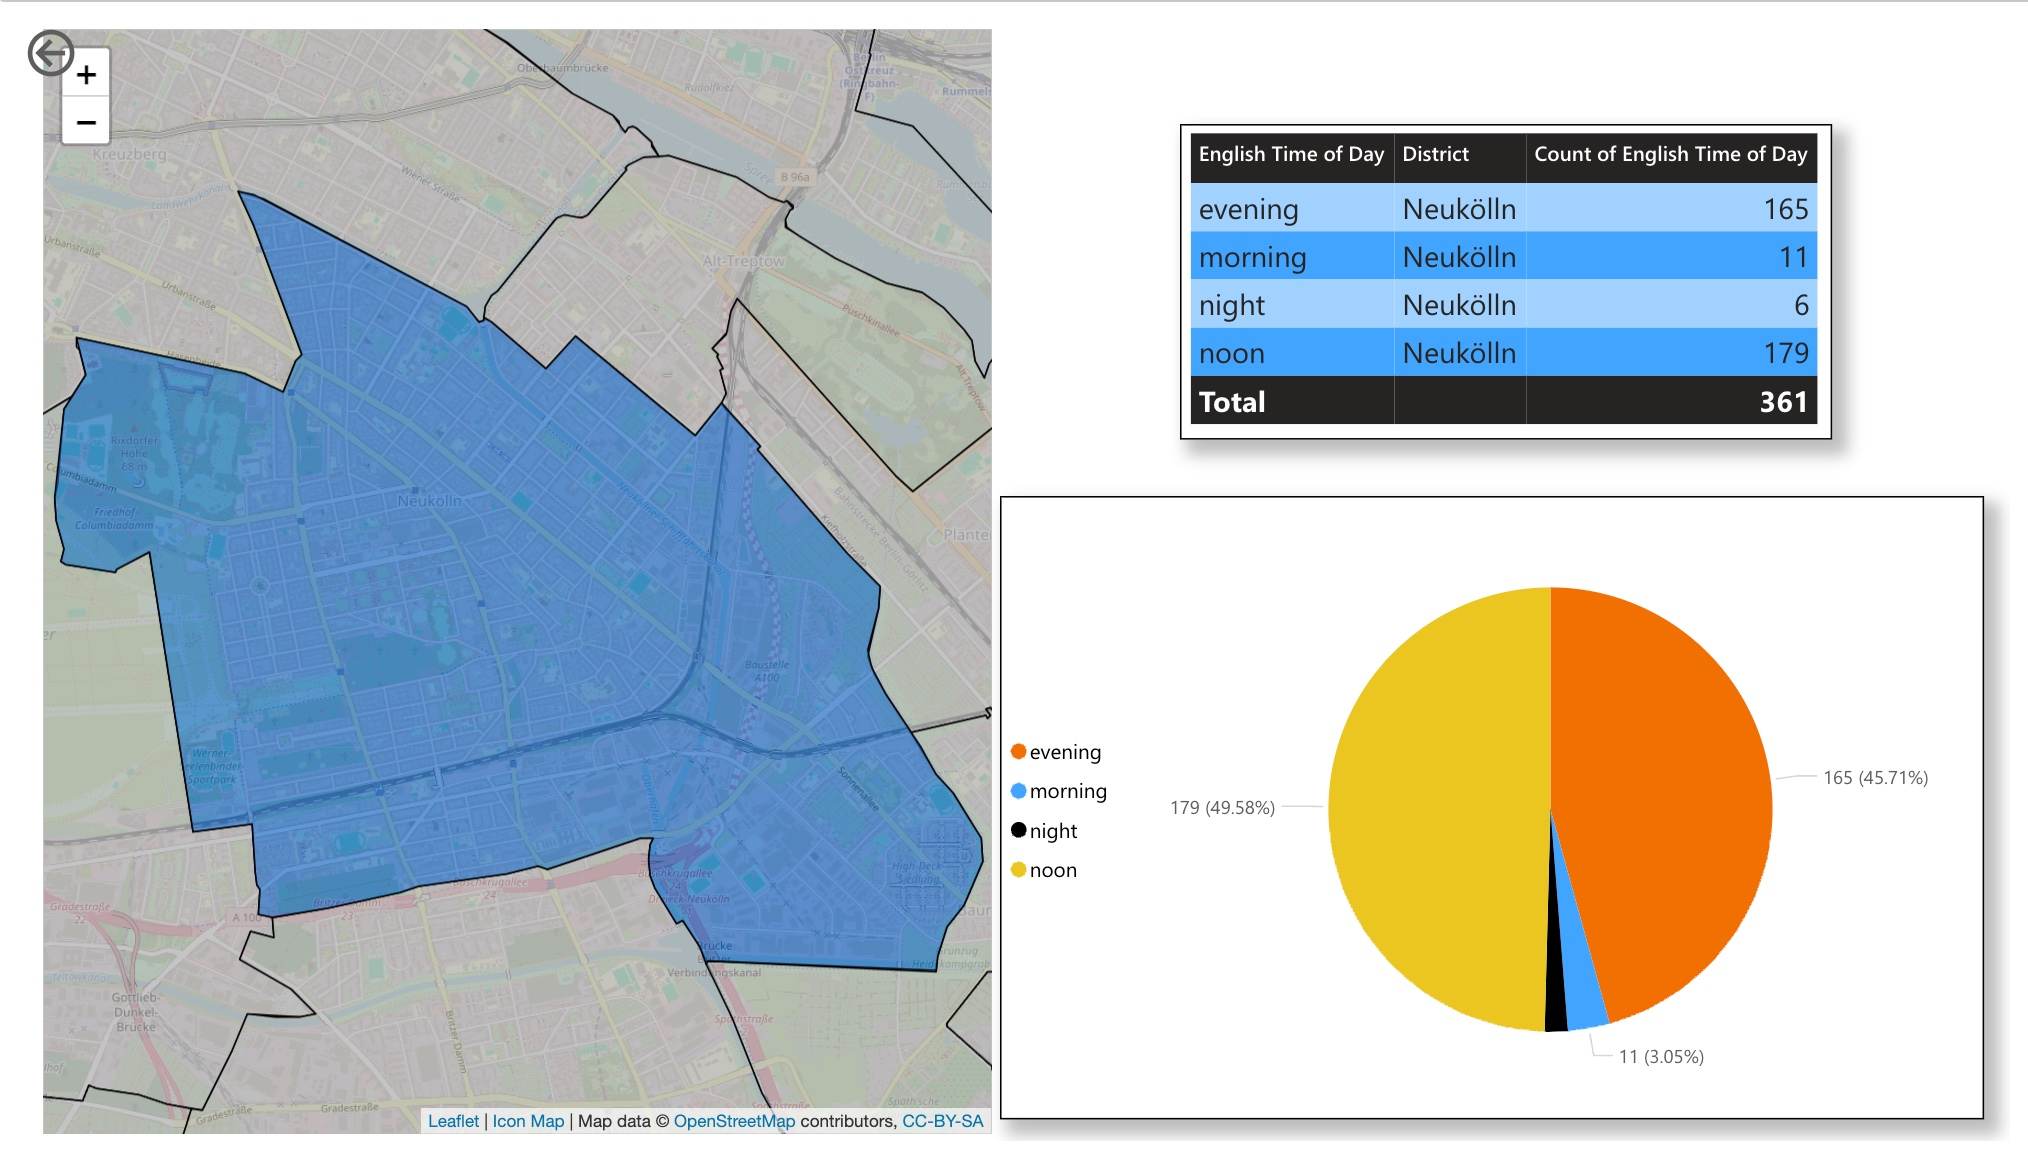
\includegraphics[width=\textwidth]{./figures/intro_rishabh/1_3.jpg}
    \caption{Caption for the image}
    \label{fig:districts}
\end{figure}

\paragraph{The possible reasons for this distribution include higher population density during noon and evening due to lunch breaks, commuting, and leisure activities. Routine activity theory suggests increased opportunities for crime when more people are in public spaces during these times. Natural surveillance is higher during busy periods, affecting crime rates. Poor lighting at night can both deter and conceal crime, but lower public activity levels also contribute to fewer incidents. Effective night-time policing or reduced public activity likely contributes to the lower crime rates at night.
}


\subsection{Word Cloud Analysis of Event Names}

\begin{figure}[!h]
    \centering
    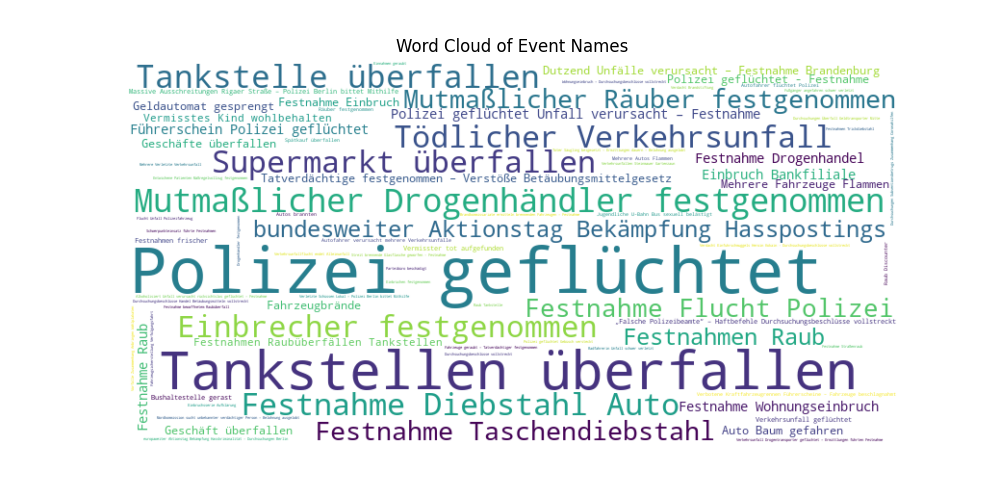
\includegraphics[width=0.8\textwidth]{./figures/intro_rishabh/Bag_of_words.png}
    \caption{Word Cloud of Event Names}
    \label{fig:wordcloud}
\end{figure}

The word cloud shows a representation of the most frequently occurring terms related to crime and harassment events in Berlin. Prominent phrases such as \textit{"Polizei geflüchtet"} (police fled), \textit{"Tankstellen überfallen"} (gas stations robbed), \textit{"Mutmaßlicher Drogenhändler festgenommen"} (suspected drug dealer arrested), and \textit{"Tödlicher Verkehrsunfall"} (fatal traffic accident) indicate the types of incidents commonly reported.

The frequent appearance of terms like \textit{"Festnahme"} (arrest) and \textit{"Überfallen"} (robbed) shows the recurring nature of criminal activities requiring police intervention. Locations such as \textit{"Tankstelle"} (gas station) and \textit{"Supermarkt"} (supermarket) appear often, suggesting these are common targets for theft and robbery. Additionally, the word \textit{"Verkehrsunfall"} (traffic accident) highlights the prevalence of serious traffic incidents, some of which have fatal consequences.

Several factors might explain these patterns. Economic disparities and social inequalities can drive individuals toward criminal activities, such as robbery and drug trafficking, as means of survival or profit. Urban areas, with their high population density, offer more opportunities for such crimes and provide anonymity for offenders.

The frequent mention of law enforcement actions, such as arrests, reflects an active police presence and effective reporting mechanisms in Berlin. This indicates a responsive legal system aimed at addressing and mitigating crime promptly. The high frequency of traffic accidents could be attributed to dense traffic conditions, inadequate infrastructure, or reckless driving behaviors common in metropolitan areas.

Overall, the word cloud offers a snapshot of the crime landscape in Berlin, highlighting key concerns and the importance of ongoing efforts in law enforcement and social policy to address the underlying causes of crime and enhance public safety.